\chapter{Zero Finding}\label{c-zero}

Almost every interesting problem in mathematics can be reduced to trying to find the zeros of a function.  The next several classes will be spent examining how we find zeros.  In general, you cannot explicitly solve for the zeros so you need to make iterative procedures to find them.  Today we will look at two methods: bisection and Newton's method.

\section{Bisection}
Bisection is a nice method in that it is guaranteed to converge and you can state exactly how many iterations it will take.  The idea of the bisection method is to pick an interval where a root is guaranteed to exist.  This is done by making the sign of the function different on the two ends of the interval.

\begin{figure}[h]
\begin{center}
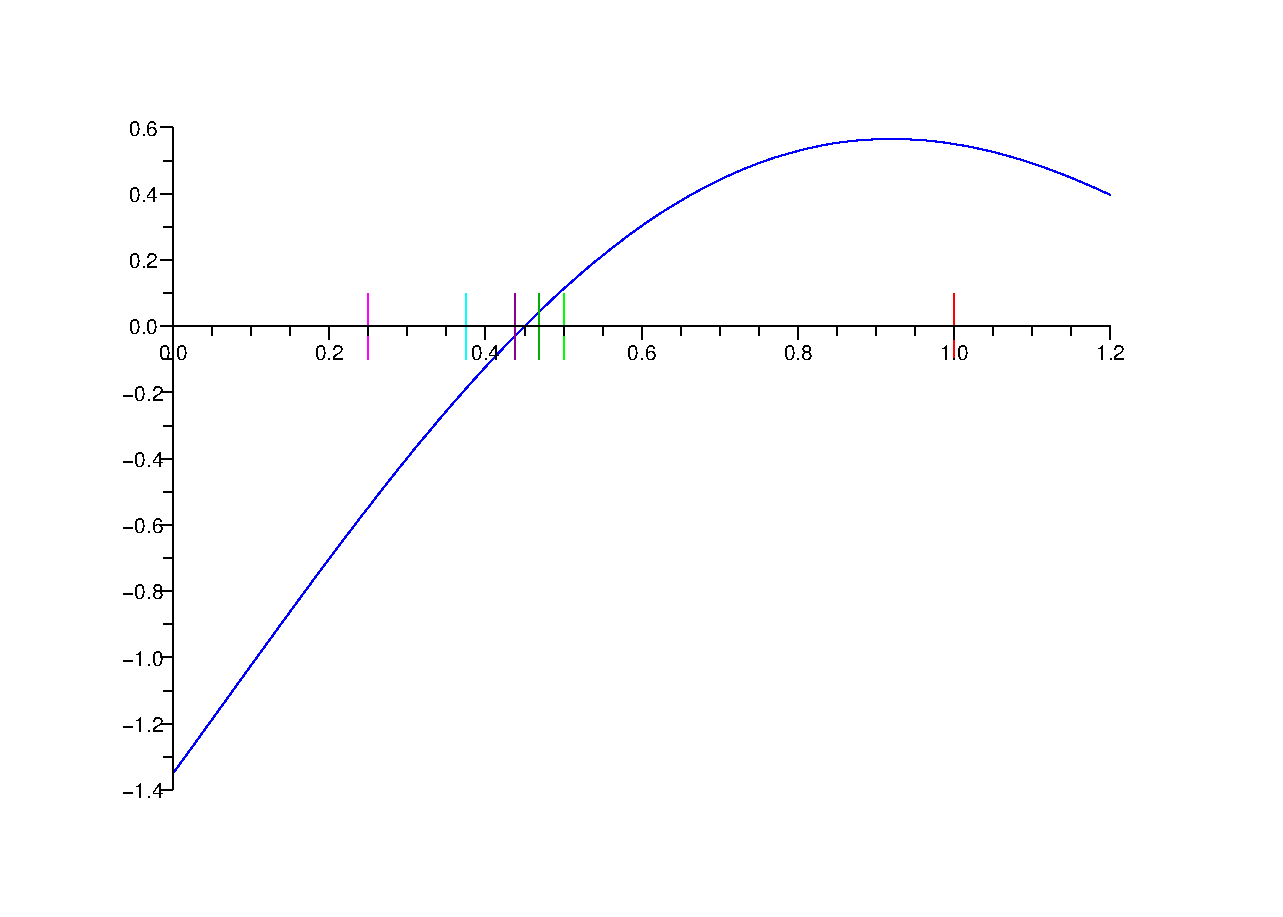
\includegraphics[width=4in]{bisection.eps}
\end{center}
\caption{Several iterations of Bisection on $f(x)=(x+1)(x-.45)(x-1.5)(x-2)$}
\label{f-bisection}
\end{figure}

For instance consider the function in Figure~\ref{f-bisection}.  The interval we start with is $[0,1]$ and it is marked by red lines.  We then calculate the midpoint (.5 marked by the light green line) and check which of the new intervals ( $[0,.5]$ or $[.5,1]$) has the zero in it (by checking which interval has a sign change).  In this case the next interval is [0,.5].  We then halve the interval again and continue.  The next several intervals marked on the plot are $[.25,.5]$, $[.375,.5]$, $[.4375,.5]$, and finally $[.4375,.46875]$.

\section{Newton's Method}

Newton's Method essentially is an algebraic re-writing of the tangent line of a function at a point.  Let the function we are trying to find the zero of be denoted by $f(x)$ and the point be $x_i$.  We know that the slope of the tangent line has to be the same as the slope of the graph at the point $x_i$, thus the tangent line is $y=f'(x_i)x+b$.  We can find $b$ by noting the line passes through $(x_i,f(x_i))$, so
\beqn
f(x_i) &=& f'(x_i)x_i+b \\
b &=& f(x_i)-f'(x_i)x_i.
\eeqn
The tangent line is thus given by $y=f'(x_i)(x-x_i)+f(x_i)$.  We are trying to find the zeros of the function $f(x)$ and the tangent line approximates the function so we want to find the point where the tangent line intercepts the x-axis.
\beqn
0 &=& f'(x_i)(x_{i+1}-x_i)+f(x_i) \\
0 &=& x_{i+1}-x_i+\frac{f(x_i)}{f'(x_i)} \\
x_{i+1} &=& x_i-\frac{f(x_i)}{f'(x_i)}
\eeqn
Newton's methods is thus the next estimate of the root is $x_{i+1}=x_i-\frac{f(x_i)}{f'(x_i)}$.  We can see this graphically in Figure~\ref{f-newton}.  Newton's method for $f(x)=x^2$ is thus $x_{i+1}=x_i-\frac{x_i^2}{2x_i}$ or $x_{i+1}=\frac{x_i}{2}$  The first estimate is $x_0=2$, the next is $x_1=1$, then $x_2=.5$ and finally $x_3=.25$.  Notice that the limit is zero as desired, and we can get as close as we want by repeating the method until $x_{i+1}-x_i<tol$, where $tol$ is some tolerance we select.

\begin{figure}[h]
\begin{center}
\includegraphics[width=5.5in]{newtonfig.eps}
\end{center}
\caption{Three iterations of Newton's Method on $f(x)=x^2$}
\label{f-newton}
\end{figure}

We can then use Taylor's formula to obtain an error bound.  Let $\alpha$ be the actual value of the root.
\beqn
e_{n+1} &=& \alpha-x_{n+1} \\
&=& \alpha-\left(x_n-\frac{f(x_n)}{f'(x_n)}\right) \\
&=& e_n+\frac{f(\alpha)-e_nf'(\alpha)+\frac{e_n^2}{2}f''(\zeta)}{f'(x_n)}
\eeqn
First, $\zeta$ is a point between $\alpha$ and $x_n$.  Second, since $\alpha$ is a root, $f(\alpha)=0$.
\beqn
e_{n+1} &=& e_n+\frac{f(\alpha)-e_nf'(\alpha)+\frac{e_n^2}{2}f''(\zeta)}{f'(x_n)} \\
&=& e_n+\frac{-e_nf'(\alpha)+\frac{e_n^2}{2}f''(\zeta)}{f'(x_n)} \\
&=& e_n\left(1-\frac{f'(\alpha)}{f'(x_n)}\right)+e_n^2\frac{f''(\zeta)}{2f'(x_n)} \\
&=& e_n\frac{f'(x_n)-f'(\alpha)}{f'(x_n)}+e_n^2\frac{f''(\zeta)}{2f'(x_n)}
\eeqn
When $x_n$ is close to $\alpha$ then $f'(x_n)-f'(\alpha)\approx 0$, so
\beqn
e_{n+1} &=& e_n^2\frac{f''(\zeta)}{2f'(x_n)} \\
&=& e_n^2C.
\eeqn
When we are close to the root, the error is dropping off as a square, thus Newton's method has quadratic convergence.


\section{Secant}
Newton's Method requires the knowledge of the first derivative of the function.  Often the derivative is very complicated to evaluate and will take a long (relatively anyway) time to do so.  In many cases the first derivative may not be available.  In some cases it might not even exist at all points in the interval of interest.  Even when it is available it could be near zero which would cause numerical problems in evaluating it, even if it is in the region of convergence.  For all of these regions a new method was devised, which drew on the material leading up to calculus.

Recall that the tangent line was found as the limit of a series of secant lines.  We can say that the derivative can thus be approximated by
\beqn
f(x)\approx\frac{f(x_{1})-f(x_{2})}{x_{1}-x_{2}}.
\eeqn
Thus if we know two points, we can approximate the function by a straight line between them and use the x-intercept as the next point to evaluate.  We now need two points instead of one and a derivative.  We refer to this as a two-point method because of the need of multiple points.  We will need two estimates to begin our evaluation.  Given two initial guesses, $x_{0}$ and $x_{1}$, the slope, $m$, is given by
\beqn
m=\frac{f(x_{1})-f(x_{0})}{x_{1}-x_{0}}.
\eeqn
Using this we find the next point, $x_{2}$ by using the point-slope form of a line
\beqn
f(x_{2})-f(x_{1}) & = &
  \frac{f(x_{1})-f(x_{0})}{x_{1}-x_{0}}(x_{2}- x_{1}) \\
x_{2}- x_{1} & = &
  \frac{x_{1}-x_{0}}{f(x_{1})-f(x_{0})}(f(x_{2})-f(x_{1})) \\
x_{2} & = &
  x_{1}-f(x_{1})\frac{x_{1}-x_{0}}{f(x_{1})-f(x_{0})}.
\eeqn
We thus have the equation for the next estimate:
\beq
x_{n+1} =
  x_{n}-f(x_{n})\frac{x_{n}-x_{n-1}}{f(x_{n})-f(x_{n-1})}. \label{eq-sec1}
\eeq
Note that you can store the previous function evaluation and then you will not need to do two function evaluations per iteration.

Now we want to calculate the error.  To do this we will subtract
eq~\ref{eq-sec1} from $\alpha=\alpha$.
\beqn
e_{n+1} & = & \alpha - x_{n+1} \\
  & = & \alpha -
    \left(x_{n}-f(x_{n})\frac{x_{n}-x_{n-1}}{f(x_{n})-f(x_{n-1})}\right) \\
  & = & \alpha -\frac{f(x_{n})x_{n-1}-f(x_{n-1})x_{n}}{f(x_{n})-f(x_{n-1})} \\
  & = & \frac{f(x_{n})(\alpha -x_{n-1})-f(x_{n-1})(\alpha -x_{n})}
       {f(x_{n})-f(x_{n-1})} \\
  & = & \frac{f(x_{n})e_{n-1}-f(x_{n-1})e_{n}}{f(x_{n})-f(x_{n-1})} \\
  & = & e_{n} e_{n-1}\frac{\frac{f(x_{n})}{e_{n}}-\frac{f(x_{n-1})}{e_{n-1}}}
       {f(x_{n})-f(x_{n-1})} \\
  & = & e_{n} e_{n-1}\frac{\frac{f(x_{n})}{e_{n}}-\frac{f(x_{n-1})}{e_{n-1}}}
       {x_{n}-x_{n-1}}\frac{x_{n}-x_{n-1}}{f(x_{n})-f(x_{n-1})} \\
  & \approx & e_{n} e_{n-1}\frac{\frac{f(x_{n})}{e_{n}}-\frac{f(x_{n-1})}{e_{n-1}}}
       {x_{n}-x_{n-1}}\frac{1}{f'(\alpha)}
\eeqn
We need to evaluate $\frac{f(x_{n})}{e_{n}}$, so we will use Taylor's Theorem for $f(x)$ evaluated at $\alpha$.  We find that
\beqn
\frac{f(x_{n})}{e_{n}} & = &
\frac{f(\alpha)+(\alpha-x_{n})f'(\alpha)+\frac{1}{2}
  (\alpha-x_{n})^{2}f''(\alpha)+{\cal O}((\alpha-x_{n})^{3})}{e_{n}} \\
& = &
\frac{e_{n}f'(\alpha)+\frac{1}{2}e_{n}^{2}f''(\alpha)
   +{\cal O}(e_{n}^{3})}{e_{n}} \\
& = &
f'(\alpha)+\frac{1}{2}e_{n}f''(\alpha)+{\cal O}(e_{n}^{2})
\eeqn
Resuming our evaluation of $e_{n+1}$ we find
\beqn
e_{n+1}
  & \approx & e_{n} e_{n-1}\frac
  {f'(\alpha)+\frac{1}{2}e_{n}f''(\alpha)+{\cal O}(e_{n}^{2})
  -f'(\alpha)-\frac{1}{2}e_{n-1}f''(\alpha)+{\cal O}(e_{n-1}^{2})}
       {x_{n}-x_{n-1}}\frac{1}{f'(\alpha)} \\
  & = & e_{n} e_{n-1}\frac{\frac{1}{2}e_{n}f''(\alpha)
   -\frac{1}{2}e_{n-1}f''(\alpha)+{\cal O}(e_{n-1}^{2})}
       {x_{n}-x_{n-1}}\frac{1}{f'(\alpha)} \\
  & = & e_{n} e_{n-1}\frac{\frac{1}{2}(e_{n}-e_{n-1})f''(\alpha)
   +{\cal O}(e_{n-1}^{2})}{x_{n}-x_{n-1}}\frac{1}{f'(\alpha)} \\
  & = & e_{n} e_{n-1}\frac{\frac{1}{2}(x_{n}-x_{n-1})f''(\alpha)
   +{\cal O}(e_{n-1}^{2})}{x_{n}-x_{n-1}}\frac{1}{f'(\alpha)} \\
  & = & e_{n} e_{n-1}(\frac{1}{2}f''(\alpha)
   +{\cal O}(e_{n-1}^{2}))\frac{1}{f'(\alpha)} \\
  & \approx & e_{n}e_{n-1}\frac{f''(\alpha)}{2f'(\alpha)} \\
  & \approx & e_{n}e_{n-1}M.
\eeqn
This is similar to Newton's method which suggests that
\beqn
  e_{n+1}=Ae_{n}^{c},
\eeqn
which implies
\beqn
  e_{n} &=& Ae_{n-1}^{c} \\
  A^{-c^{-1}}e_{n}^{c^{-1}} &=& e_{n-1}.
\eeqn
Substituting and collecting terms we find
\beqn
(Ae_{n}^{c}) &=& (e_n)(A^{-c^{-1}}e_{n}^{c^{-1}})M \\
A^{1+c^{-1}}M^{-1} &=& e_n^{1-c+c^{-1}} \\
B &=& e_{n}^{1-c+c^{-1}}.
\eeqn
Since the left hand side is a constant the exponent must be zero, because $e_n$ is a variable.  This means
\beqn
0 &=& 1-c+c^{-1} \\
&=& c^2-c-1 \\
c &=& \frac{1\pm\sqrt{1+4}}{2},
\eeqn
or $c$ must be the golden ratio.  This implies that the secant method converges superlinearly.

\section{Regula Falsi}


\section{Fixed Points}
A fixed point is a point in the domain of a function, which maps its
domain back into its domain, that satisfies $\alpha=C(\alpha)$.
Since $\alpha$ does not change when it is mapped by the function it is
fixed, hence the name.  We need to look at what
the idea that underlies fixed points: contractions.  A contraction
$y=C(x)$, is a mapping from a closed interval in $X$ into another closed
interval in $Y$ with the property that for some $b=C(a)$ (usually $a$
and $b$ are both the origin but it is not required), $\|\cdot\|_{x}$
a norm on $X$, and $\|\cdot\|_{y}$ a norm on $Y$ we have:
\beqn
\| x-a\|_{x} > \| y-b\|_{y} = \| C(x)-C(a)\|_{y}
\eeqn
for all $x\in X$ and $y\in Y$.  Usually we have $X$ and $Y$ are $\Re$
and $a=b$, which gives us that $|x-a|>|C(x)-a|$.  Take the derivative of both
sides and we see
\beqn
1>|C'(x)|.
\eeqn
This brings up a key point, we must have that the magnitude of the
function's slope is less than 1.  If you think about this it makes
sense, as for slope magnitudes greater than one there will be growth
and we are looking a funcions which shrink things.  While this is a
simple idea, it has many profound implications.  The book proves
nicely how the uniqueness of solution, convergence, etc..  One thing
that should be highlated has to do with rate of convergence.  Given a
contraction defined on an interval $[a,b]$ with some point, $\alpha =
C(\alpha)\in[a,b]$ called a fixed point, we can define the iteration
$x_{n+1}=C(x_{n})$.  We then have (using the mean value theorem)
\beqn
\alpha-x_{n+1}
 & = & C(\alpha)-C(x_{n}) \\
 & = & C'(d)(\alpha-x_{n}) \\
|\alpha-x_{n+1}|
 & < & |\alpha-x_{n}|.
\eeqn
We have linear convergence from this.  Consider the following paradox.

Let a function $g(x)$ be defined by
\beqn
g(x)=x-\frac{f(x)}{f'(x)}
\eeqn
and let $f(x)$ have a single root in some interval $[a,b]$.  From the
book we know this must have a fixed point in the interval and the
iteration $x_{n+1}=g(x_{n})$ will converge to the fixed point.  This
method thus has linear convergence from what we have proven above.
This iteration is Newton's Method though, so it has Quadratic
convergence.  What gives?  The convergence of a fixed point algorithm
is at least linear but it can be better if $C'(\alpha)=0$.  Notice
that the derivative of $g(x)$ is given by
\beqn
g'(x) & = & 1-\frac{(f'(x))^{2}-f(x)f''(x)}{(f'(x))^{2}} \\
      & = & \frac{f(x)f''(x)}{(f'(x))^{2}}.
\eeqn
Note that for $x=\alpha$ we trivially have that $g'(\alpha)=0$, which
satisfies our requirement for faster convergence.

How can I get a function $g(x)$ that satisfies the requirements?
Many ways exist but consider the following.  For a function $f(x)$ with
a zero at $x=\alpha$ in an interval $[a,b]$, that has
$\beta=\max_{x\in[a,b]}|f'(x)|$, we define the iteration
\beqn
x_{n+1}=x_{n}-\gamma sign(f'(x_{n}))f(x_{n})
\eeqn
with $0<\gamma\beta<2$.  We then see that
\beqn
g(x) & = & x-\gamma sign(f'(x))f(x) \\
g'(x) & = & 1-\gamma sign(f'(x))f'(x) \\
      & = & 1-\gamma |f'(x)|
\eeqn
and thus $1>g'(x)>-1$.  Note that if we choose $\gamma$ such that
$0<\gamma\beta<1$ then $1>g'(x)>0$ and the sequence
$\{x_{i}\}_{i=0}^{\infty}$ converges to $\alpha$ from one side (no
alternating).  The parameter $\gamma$ is refered to as the {\bf step
size}.  As a final note, we can use Aitken's $\Delta^{2}$ method as
outlined in the book to refine the estimate $x_{n}$.  Replace $\alpha$
with $\hat{x}_{n}$ and you have a refinement and acceleration method
that will work on any linearly convergent algorithm.  It can thus be
used on general fixed point methods.

Homework
4.3: 6, 13
\newpage
\section{Continuation Methods}
One of the essential problems in root finding is to find a good place
to start.  We have spoken about the progressively doubling intervals
till we find a sign change.  I mentioned this was not the fastest or
best, but would work.  I wanted to give you what I think is one of the
best.  It is refered to as a continuation method or sometimes a
homotopy.

A homotopy, $h$, is a continuous connection between two functions, $f$ and
$g$, that maps one space, $X$, to another, $Y$:
\beqn
h:[0,1]\times X\rightarrow Y
\eeqn
such that $h(0,x)=g(x)$ and $h(1,x)=f(x)$.  Two simple homotopies we will
use are listed below.
\begin{enumerate}
\item
\beqn
h(\lambda,x)=\lambda f(x)+(1-\lambda)g(x)
\eeqn
\item
\beqn
h(\lambda,x) & = & \lambda f(x)+(1-\lambda)(f(x)-f(\alpha_{0})) \\
             & = & f(x)-(1-\lambda)f(\alpha_{0})
\eeqn
\end{enumerate}
The first one is the most general.  Assume we want to find the roots
of $f$, but we know the roots of $g$.  By picking a sequence of
$\lambda$ values from zero to one, we will slowly make the roots move
from the known positions of $g$ to the unknown positions of $f$.  We
usually try to pick $g$ so it has the same number of roots as the
function $f$.

The second method is a frequently used one if I don't want to find a
function $g$.  We are in essence biasing the original fucntion so that
at $\alpha_{0}$ the homotopy has a root for $\lambda=0$.  This gives a nice
starting point.  The following theorem tells us when this will work.

\begin{theorem}[Ortega and Rheinboldt]
If $f:\REn\rightarrow\REn$ is continuously differentiable and if
$\|[f'(x)]^{-1}\|\leq M$ on $\REn$, then for any $\alpha_{0}\in\REn$ there
is a unique curve $\{\alpha(\lambda):0\leq\lambda\leq 1\}$ in $\REn$ such
that $f(\alpha(\lambda))-(1-\lambda)f(\alpha_{0})=0$, with $0\leq\lambda\leq
1$.  The function $\lambda\mapsto \alpha(\lambda)$ is a continuously
differentiable solution to the initial value problem
$\alpha'=-[f'(\alpha)]^{-1}f(\alpha_{0})$, where $\alpha(0)=\alpha_{0}$.
\end{theorem}

Essentially this tells us if $f$ is smooth and the first derivative
doesn't get too close to zero then you can use this start one of our
rootfinding methods, for instance Newton's Method.  Often this method
is solved by using a numerical integration technique which we will
cover in a few weeks.  For instance if Euler's method is used then it
turns out to generate Newton's Method in $\lambda$!

\section{Multiple Roots}
One thing that always caused us problems in all our methods is
multiple roots.  I will present a simple technique for handling this
case.  Let our function, $f$, with root of multiplicity, $2$, be given
by
\beqn
f(x)=(x-\alpha)^{2}f_{1}(x),
\eeqn
where $f_{1}$ has no root at $\alpha$.  Take the derivative of $f(x)$
to obtain
\beqn
f'(x) & = & (x-\alpha)f_{1}(x)+(x-\alpha)^{2}f'_{1}(x) \\
      & = & (x-\alpha)(f_{1}(x)+(x-\alpha)f'_{1}(x)) \\
      & = & (x-\alpha)f_{2}(x),
\eeqn
where $f_{2}(x)$ has no root at $\alpha$.  We now have a funcition
with a single root at the same place that the original function had a
double root.  This can be done for higher multiplicity roots, and
does not require knowing $\alpha$ as we are taking the derivative then
finding $\alpha$ using one of our techniques.

\section{Sensitivity}
This is refered to as stability of the roots in the books, but it is
more closely related to the sensitivity of a differential equation to
perturbations in its coefficients.  For instance, consider a famous
problem due to Wilkinson.
\begin{problem}[Wilkinson]
Find the roots of the polynomial $f(x)$ given by
\beqn
f(x) & = & (x-1)(x-2)\cdots(x-20) \\
     & = & x^{20}-210x^{19}+\cdots +20!
\eeqn
The roots are clearly one through twenty.  Perturb the coefficient
$-210$ to $-210-2^{-23}$.  The change is in one coefficient only, and
that in the $7^{th}$ decimal place.  The roots are now
\begin{tabular}{l c c}
$1.000000000$ & $6.000006944$ & $10.095266145\pm 0.643500904j$ \\
$2.000000000$ & $6.999697234$ & $11.793633881\pm 1.652329728j$ \\
$3.000000000$ & $8.007267603$ & $13.992358137\pm 2.518830070j$ \\
$4.000000000$ & $8.917250249$ & $16.730737466\pm 2.812624894j$ \\
$4.999999928$ & $20.846908101$ & $19.502439400\pm 1.940330347j$
\end{tabular}
The problem is not roundoff.  The roots of high-order coefficients can
be extremely sensitive to changes in the coefficients.  This is a
problem particularly when the coefficients are experimentally
determined.
\end{problem}
